\begin{abstract}

Here we define paradata as the data that describes the generation of data.
In genetic epidemiology, the data generated is mostly the results 
of an analysis (e.g. predicting a person having a disease),
as done by computer code.
In such context, paradata is usually the scientific paper that
describes what the computer code does.
However, this has the unrealtistic 
assumption that there is a perfect match between the paper and the code.
In this chapter it is argued that the source code should should be supplied,
as this is the true paradata: if the paper and code disagree, it is the
code that has generated the results.
The chapter concludes by some rules how to allow code to serve as paradata,
and hence allowing computational research to be truly reproducible.

\end{abstract}

{\bf Keywords:} paradata, reproducible research, code, software,
FAIR data, computational research, Open Science, DevOps, best practices,
genetic epidemiology

%%%%%%%%%%%%%%%%%%%%%%%%%%%%%%%%%%%%%%%%%%%%%%%%%%%%%%%%%%%%%%%%%%%%%%%%%%%%%%%%
\section*{Definitions}
%%%%%%%%%%%%%%%%%%%%%%%%%%%%%%%%%%%%%%%%%%%%%%%%%%%%%%%%%%%%%%%%%%%%%%%%%%%%%%%%

\begin{table}[h]
  \begin{tabular}{lll}
    Term      & Definition                                            & Example                                                         \\
    \hline
    Data      & Individual facts, statistics, or items of information & A SNP that has a significant association                        \\
    Genotype  & The DNA allele at a certain location                  & AA, AC, CG, GT, ...                                             \\
    Paradata  & Data that describes the generation of data            & The code to conclude that a SNP has a significant association   \\
    Phenotype & How an organism looks like in the broadest sense      & The concentration of IL6RA in the blood                         \\
    Metadata  & Data that provides information about other data       & The article that describes an experiment                        \\
    Trait     & A phenotype                                           & The concentration of IL6RA in the blood                         
  \end{tabular}
\end{table}

%%%%%%%%%%%%%%%%%%%%%%%%%%%%%%%%%%%%%%%%%%%%%%%%%%%%%%%%%%%%%%%%%%%%%%%%%%%%%%%%
\section{Introduction}
%%%%%%%%%%%%%%%%%%%%%%%%%%%%%%%%%%%%%%%%%%%%%%%%%%%%%%%%%%%%%%%%%%%%%%%%%%%%%%%%

% This section has paragraph headers. This helps me, the author,
% to focus the contents of my paragraphs.
% In the final version of this manuscript, these will be removed.

\paragraph{Universities produce knowledge}

The currency that universities generate is knowledge, which in turn is distributed
in mostly lectures and academic papers.
Academic papers contain knowledge, either as the
report of measurements or the outcome of an experiment.
These reports are described in English, the current lingua franca of science.

\paragraph{A paper contains data and should be FAIR data}

A paper contains and/or describes data, where we define
data as 'individual facts, statistics, or items of information, often 
numeric' \cite{glossary2003oecd}.
To ensure unhampered knowledge growth, this data should [TODO: Why? Reference!] 
follow the FAIR 
principles.
The FAIR principles \cite{wilkinson2016fair} are that data should be 
[TODO: there are probably better examples]
Findable (e.g. found by web),
Accessible (e.g. DataDryad and or Zenoda), 
Interoperable (e.g. comma-separated files) 
and Reusable (e.g. work on all operating systems)

\paragraph{A paper is data and should be FAIR data}

A paper in itself is data, as it is a collection of text and
figures that we itself can do measurements upon.
Also here, a paper should be FAIR, 
[TODO: there are probably better examples]
i.e.
Findable (e.g. Google Scholar)
Accessible (e.g. view it online), 
Interoperable (e.g. written in English)
and Reusable (e.g. it is valid to cite and build upon earlier academic papers).
This paper itself will later specify the standpoint that a paper
is metadata (i.e. data about data), instead of paradata (i.e.
data that describes the collection of data)

\paragraph{For some fields, the experiment is actually run by code}

This paper focusses on research fields that uses computation
to do experiments and uses genetic epidemiology as an example.
Genetic epidemiology is a field within biology that, among 
others, measures the spread (hence 'epidemiology') 
of heritable (i.e. genetic) traits, as well as the relation
between having a certain genetic makeup and a certain trait,
where the trait can be any human property, such as weight, height,
the amount of metabolites and having a disease yes/no.

\begin{figure}[!htbp]
  \centering
  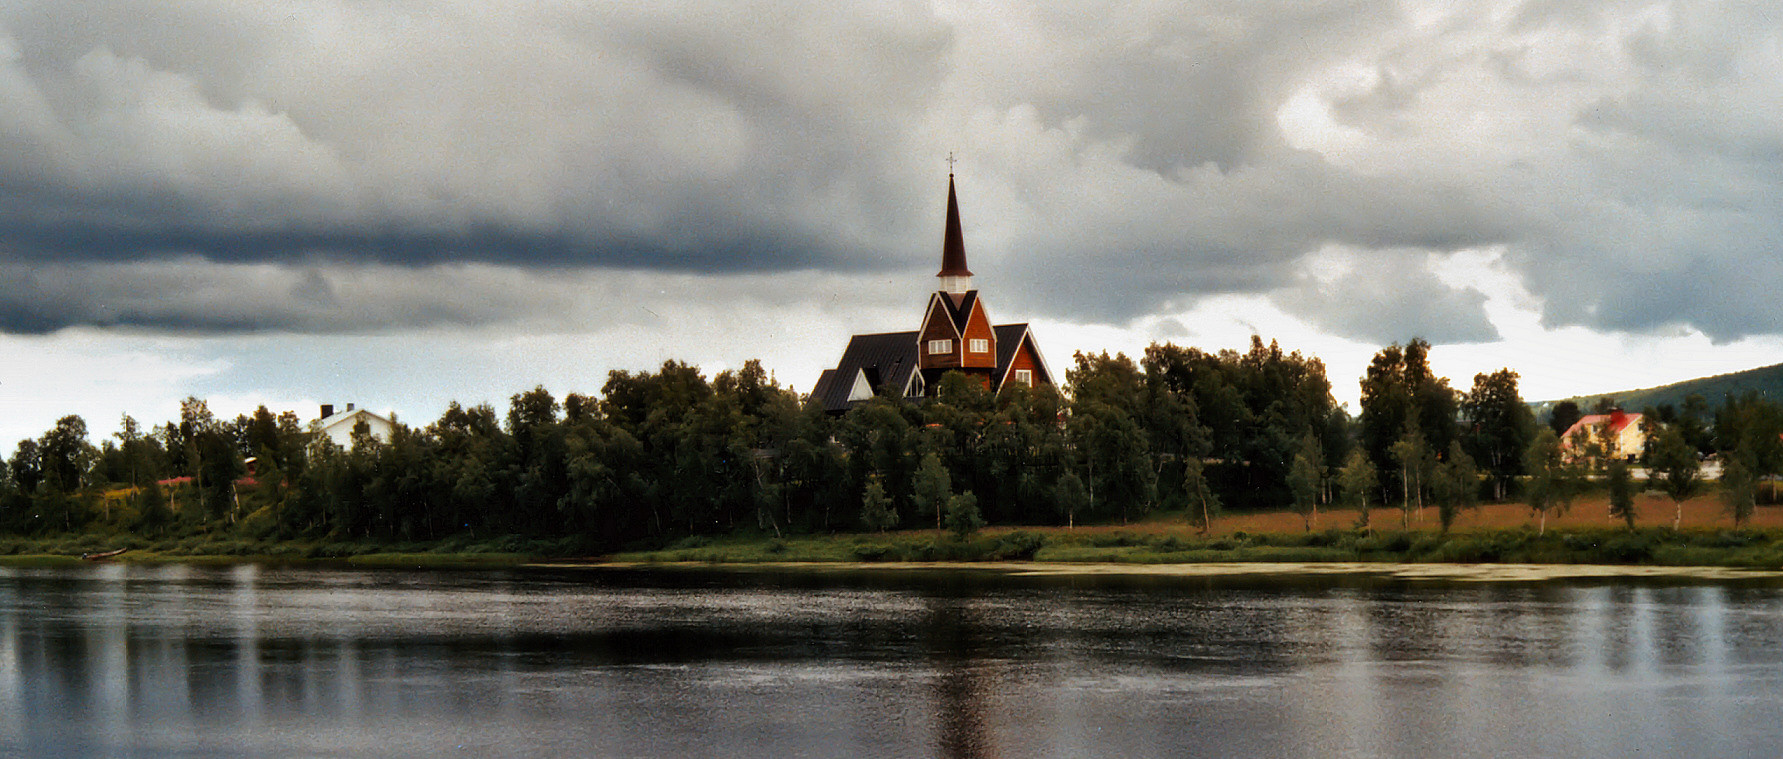
\includegraphics[width=\linewidth]{Karesuando_church.jpg}
  \caption{
    Figure F2: Picture of Karesuando's church,
    the village where the Northern Swedish Population
    Health Study started.
    From \cite{hopfner2005}
  }
  \label{fig:karesuando_church}
\end{figure}

As an example, we'll use a pseudorandomly selected paper
from [Ahsan et al., 2017]. The data used by that paper is
from a population study called the Northern Swedish Population
Health Study (NSPHS) that started in 2010 [Igl et al., 2010]. 
The approximately 1000 participants were initially mostly surveyed
about lifestyle [Igl et al., 2010] and follow-up studies
provided the type of data relevant for this paper, 
which are (1) the genetic data [Johansson et al., 2013],
(2) the concentration of certain proteins in the 
blood [Enroth et al., 2014][Enroth et al., 2015].

\begin{figure}[!htbp]
  \centering
  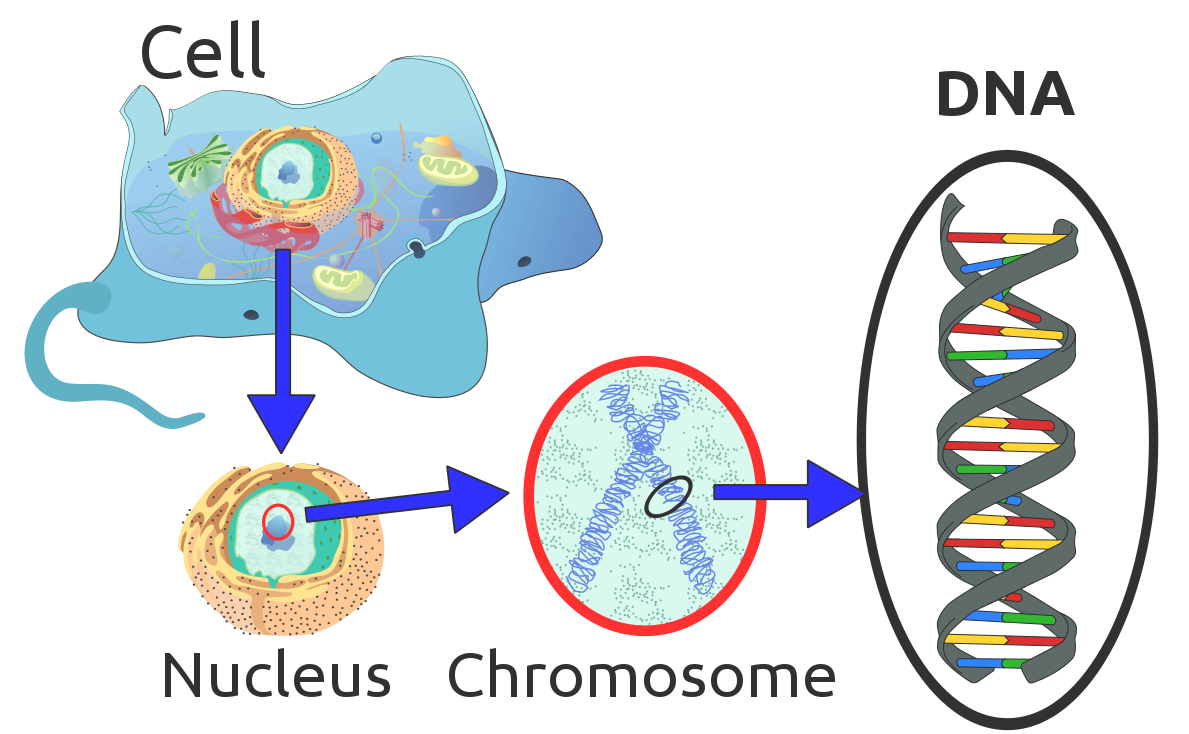
\includegraphics[width=\linewidth]{1189px-Eukaryote_DNA-en.png}
  \caption{
    Fig F3: A cell has a nucleus that contains chromosomes. 
    Each of these chromosomes (46 in humans) consist out of DNA. 
    DNA itself conists out of 4 nucleotides, 
    as depicted by the horizontal sticks 
    with the colors red, yellow, green and blue.
    From [Sponk et al., 2012]
  }
  \label{fig:eukakyote_dna}
\end{figure}

The first type of data, the (final form of the) genetic data,
consists out of single nucleotide polymorphisms (SNPs).
SNPs consist out of a name, a position and a nucleotide. 
DNA (organized into chromosomes and present in every (nucleated) cell, 
see figure F3) consists out of many nucleotides, of which there are four types,
called adenosine, cytosine, guanine and thyrosine, all commonly abreviated
as A, C, G and T respectively.
One SNP example is, that 'rs12133641' is a SNP located at position 154,428,283,
where some people have a certain nucleotide. In this case, 
67 percent of the people within this study have an A,
and 33 percent have a G (also from [Ahsan et al., 2017], Table S3).

\begin{figure}[!htbp]
  \centering
  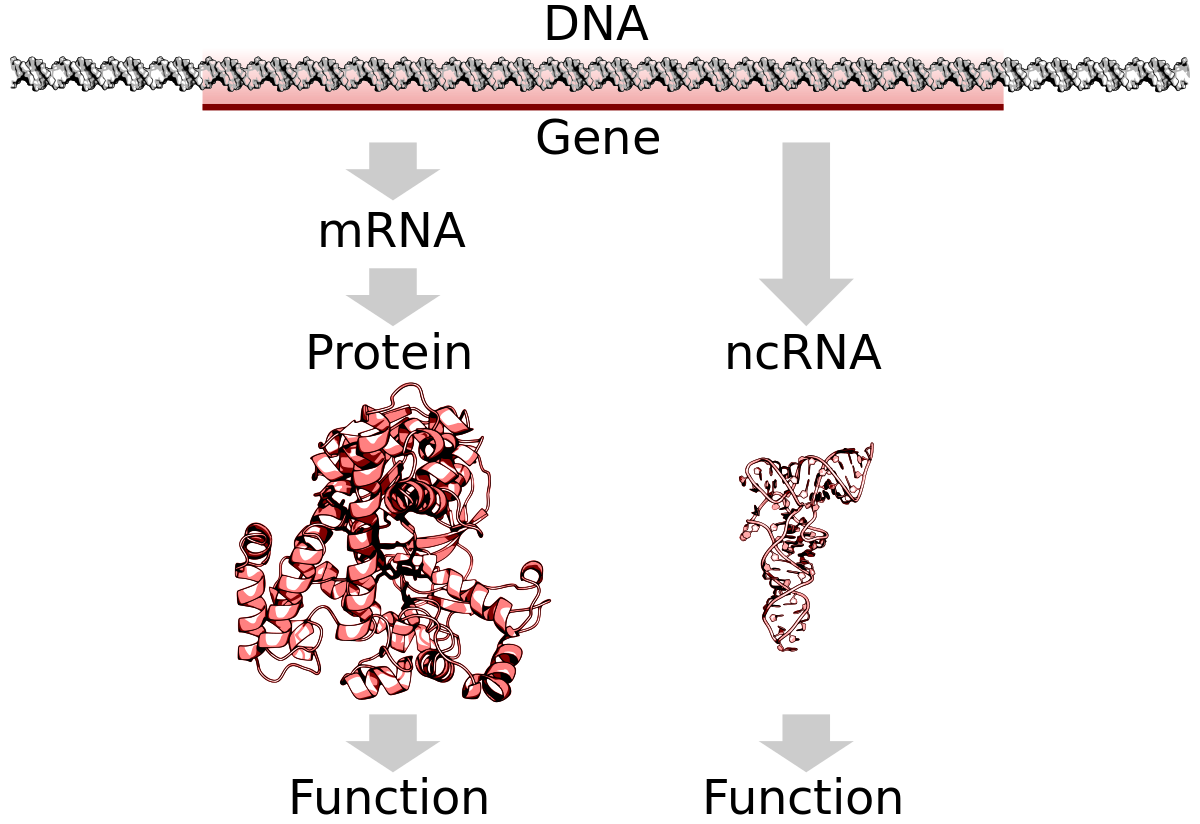
\includegraphics[width=\linewidth]{DNA_to_protein_or_ncRNA.png}
  \caption{
    Fig F5: Parts of DNA (so-called 'genes') code for proteins. 
    The DNA, that always stays put in the cell's nucleus, 
    is transcripted to messenger RNA (mRNA).
    mRNA leaves the nucleus and its code gets translated to 
    a protein sequence.
    Near the start of a gene are regions that determine the amount
    of proteins produced (not shown in figure).
    Adapted from [Shafee, 2015]
  }
  \label{fig:dna_to_protein}
\end{figure}

The second type of data are concentrations of certain proteins in the 
blood. DNA contains the code for building proteins (see Figure F5), 
as well as the rate
at which a protein is created. Some proteins end up in the blood and
their presence can be used to assess the health of an individual.
IL6RA is a protein [TODO: more info]

The field of genetic epidemiology looks -among others- for
correlations between genetic data and biological traits.
For example, figure F10 (from [Ahsan et al., 2017]) shows that
SNP rs12133641 is highly correlated (p value is 3.0 * 10e-73, 
961 individuals) with protein IL6RA. What this results does
not yet teach us, is how this correlation works, yet
figure F20 shows us the direction of the association:
the X axis shows the possible genetic make-ups (aka the genotype) of the individuals,
where 0 denotes the individuals with genotype
AA (the individual inherited one adenosine 
from his/here mother and one adenosine from his/her father), 
1.0 denotes AG (one A is inherited from one parent, 
where the G is inherited from the other parent) and 2.0 denotes GG.
From Figure F20 we can conclude that, on average,
the more guanines are inherited at that SNPs location,
the higher concentration of IL6RA can be found in a human's blood.

The amount of variance that can be explained by an association (i.e.
the R squared value) is rarely 100 percent, which means that a trait (in
this case, IL6RA concentrations) cannot be perfectly explained
from the genotype alone. As we can see in figure F20, 
43 percent of the variance can be attributed to an individuals'
genotype and additional factors, 
such as the effect
of the environment (e.g. geographic location, time of day), 
lifestyle (e.g. smoking yes/no) or having a disease (e.g. diabetes) 
are needed to explain the variation between individuals better.

\begin{figure}[!htbp]
  \centering
  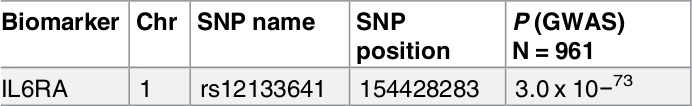
\includegraphics[width=\linewidth]{ahsan2017relative_table_2_sub.png}
  \caption{
    Figure F10 shows an example result of a genetic epideological research.
    It shows that the SNP named rs12133641 (located at position 154,428,283
    of chromosome 1) is highly correlated (p value is 3.0 * 10e-73, 
    961 individuals) to the concentration of the protein IL6RA, as measured
    in blood. The table is a simplified result from [Ahsan et al., 2017].
  }
  \label{fig:ahsan2017relative_table_2_sub}
\end{figure}


\begin{figure}[!htbp]
  \centering
  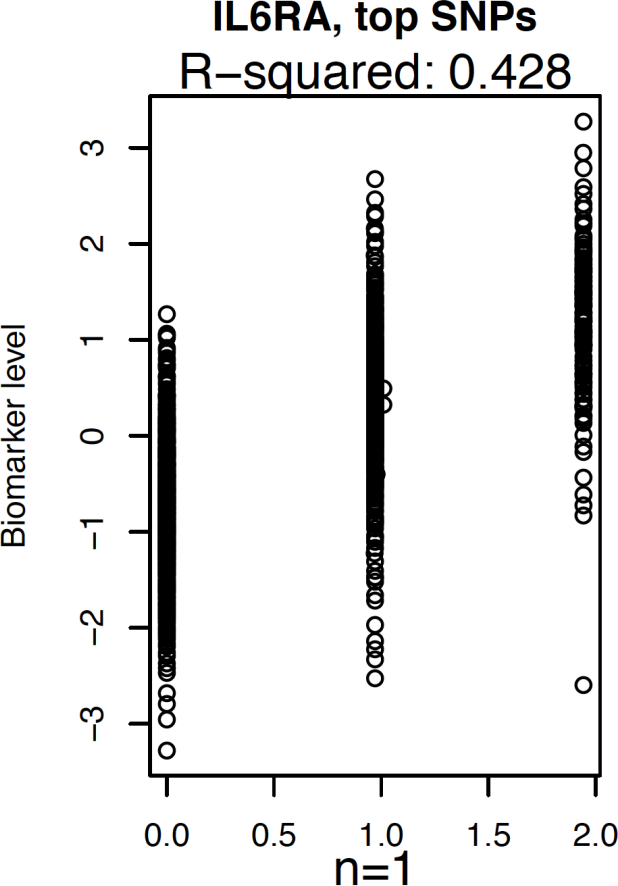
\includegraphics[width=\linewidth]{ahsan2017relative_s6.png}
  \caption{
    Figure F20: the relation between the genotype for SNP rs12133641 
    and the protein concentration of IL6RA is relatively strong.
    The X axis shows the the genotype of the individuals,
    where 0 denotes AA, 1.0 denotes AG and 2.0 denotes GG.
    The Y axis shows the concentration of the protein IL6RA 
    as found in the participants' blood. n = 1 denotes the number
    of SNPs that were determined to be involved.
  }
  \label{fig:ahsan2017relative_s6}
\end{figure}

\paragraph{The experiments within genetic epidemology works are done by code}

The experiment described above is run by code. There is no fieldwork,
nor lab-work involved. It is the researcher that writes the code,
after which the code does the work. A genetic epidemiologist that
looks for associations between genotype and phenotype,
one does not need a lab.

To **obtain** the genetic data, yes, there may be fieldwork and/or lab-work
involved. For example, a researcher needs to go into the field to take
samples (e.g. blood) of humans or other species. To analyse these samples,
a researcher needs a lab. Depending on the technique being used on
how to analyse the samples, there may be a big bioinformatics step
to aggregate the measurements into useful genetic data. 
Although this paper does not focus on the code run to 
aggragate the raw data into useful genetic data, the same arguments
can be made for that code as in the example: that code is 
the ground truth of how the raw data is collected into useful genetic data.

\paragraph{The code is the paradata for the results of an experiment}

Programming code is paradata, as it is data that describes how data is collected,
which is the definition of paradata [TODO: REF].
Programming code is data that is usually in the form of text, 
spread over one or more files, that describes the experiment.
The experiment collects the data.
The data collected is the data we call the results of an experiment.

The article is metadata, as it is data that describes other
data, which is the definition of metadata [TODO: REF]:
an article describes the
experiment and hence the programming
code in English. However, it is not the best
candidate to describe how the data is collected,
as it has a loose connection with collecting the data.
Again, if the code and article of an experiment disagree,
it is the code that actually let the data be collected.  
Instead, an article is metadata about a research.

\paragraph{Code should be published}

For science to be reproducible (a fundamental property of the scientific 
method), it is the code that should be published, instead of the
English description of what the code does (i.e. the article), if one
would have to pick one, as it is the code does the actual work.
Hence, from a knowledge management perspective, emphasis should be
put more on the preservation of code, as it is the most important actor
in an experiment.

To quote a review on reproducibility [Peng and Hicks, 2021], 
'Reproducibility is typically thwarted by a 
lack of availability of the original data and computer code'.
In the case of genetic epidemiology, it is a given that the original
data cannot be published as this data is sensitive.

\paragraph{Example of code being the ground truth}

Code should be published, as it holds the
ground truth of an experiment; it does the actual work.
The more complex the computation pipeline is, the easier it is
to have a mismatch between the article (that describes what the
code does) and the code (that actually does the work).
It is easy (tempting?) to overlook how easy it is to have a mismatch
between paper and code.

To illustrate how easy it is to get a mismatch between a paper
and the code, consider this fictional example
of a text in a paper:

> We compared the values of `x` and `y` using a one-tailed Student's T-test,
> as we expect the average value of `x` to be less than the average value of `y`.

We ignore the choices of words and style of this sentence: what is
important is the content: a one-tailed T test is performed.
Taking a look at the (in this case, the programming language R) code, 
we find the following line:

\begin{verbatim}
t.test(x, y)
\end{verbatim}

The line of code is simplified (as the result of the T test is never stored),
but the code is correct: 
`t.test` is indeed the name of an R function to do a T-test
and it is reasonable to assume that this code, when found in the code
of an article, is assumed to be correct.

Here, however, we see a mismatch between the English description and the code:
by default, the R function `t.test` does a **two**-tailed T-test.
A consequence of this fictional example is that the published p-values are
higher than needed, resulting in less significant findings, which
results in less conclusions drawn from a paper.

It is the paper that accompanies the code,
as it is the code that generates the results.
When humans are fallible and code gets bigger, the likelihood of
a mismatch between the English paper and the code increases.
But regardless of the size of the code, 
it is the code that is the ground truth.

\paragraph{Code itself has important properties}

The code of a computational experiment is
more important to preserve than the article describing
the experiment, even when both describe the experiment identically,
correctly and reproducibly. 
Here I will argue why this is the
case and the implications and best practices for knowledge preservation.
To summarize, (1) it gives an honest indication of the quality 
of a computational experiment, ....

Optionally, code can actively teach what it does.
Here, I will go into more detail of each point.

\paragraph{Example of code being convincing}

As code is paradata, as it describes how data is being collected,
it can convince (or not) that it does so correctly.
Similar to a cell biologist that can be working sterile to avoid contamination
by airborne bacteria, 
or sloppy and likelier to have contaminated samples,
code can be examplary or sloppy.

\paragraph{Code is hard to manage}

Unlike English, code is fragile in standing the test of time.
Containers can alleviate this.
Code has a limited lifetime.

\paragraph{Hosted code has important metadata}

 * Number of commits
 * Commit history
 * Code coverage
 * Objective indicator of work being done

\paragraph{Runnable code has other important features}

 * Reproduce an experiment
 * Code can teach the user, see babette
 * Build upon an experiment

%%%%%%%%%%%%%%%%%%%%%%%%%%%%%%%%%%%%%%%%%%%%%%%%%%%%%%%%%%%%%%%%%%%%%%%%%%%
\section{Conclusions}
%%%%%%%%%%%%%%%%%%%%%%%%%%%%%%%%%%%%%%%%%%%%%%%%%%%%%%%%%%%%%%%%%%%%%%%%%%%

The code that does the work in a computational experiment should
always be published together with a scholarly article.
For research to be reproducible, one ideally has access to
both the data used and the code.
In some fields, such as genetic epidemiology, the data is
sensitive, hence cannot be released,
yet there are methods being devised to run code on sensitive
data with assured privacy [Zhang et al., 2016][Azencott, 2018].

Code has additional useful information, similar to confidence intervals,
that allow a reader to gauge how much he/she trusts the results.
The most important way to determine the quality of code
is the amount of unit tests.
When following a set of best practices, such as DevOps, TDD, Agile,
writing unit tests is an essential 
part in writing code.
The amount of unit tests is an honest signal 
for code correctness (i.e. it does what it is supposed to do, as opposed
to 'it does something').
In academia, to uncover the truth, code correctness is essential.
To make a comparison with cell biologists, where working
sterile is essential to have the correct results,
unit tests allow a computational biologist to have the same.

Code is harder to preserve than an English text.

Although code is the primary actor in computational experiments,
there is no incentive to submit code alongside a publication.
Most academic journal do not require authors to submit their code,
nor it the submitted code peer reviewed.

Although the code of computation experiments can be archived well, 
there is no incentive to do so.

Although a runnable version of a computation experiment can be archived well, 
there is no incentive to do so.

%%%%%%%%%%%%%%%%%%%%%%%%%%%%%%%%%%%%%%%%%%%%%%%%%%%%%%%%%%%%%%%%%%%%%%%%%%%
\section{Discussion}
%%%%%%%%%%%%%%%%%%%%%%%%%%%%%%%%%%%%%%%%%%%%%%%%%%%%%%%%%%%%%%%%%%%%%%%%%%%

\paragraph{Definition}

Code may or may not be paradata, depending on how the definition
is interpreted.
Here we repeat the definition of 'paradata' and discuss 
its (numbered) constituents.
This paper defined paradata as 'data (1) about the collecting (2) of the data (3)',
where (1) code must be seen as data, (2) downloading raw data
and doing calculations must be seen as collecting, and (3) the
results of an experiment must be seen as data.
This paper argues, that (1) code is data in the form of text spread
over one or more files, that has useful measurable properties, 
(2) downloading raw datas and doing calculations, such as a T-test,
does describe how the bits and pieces of an end result is collected,
and (3) an experimental results is data, as it can be measured and
used as the raw data of a next experiment.

\paragraph{The drawbacks of publishing code}

Publishing code may be disadvantageous for an author.
For science, yes, as this allows reproducible research.
For an author, publishing code alongside an experiment opens up
the possibily to receive questions regarding that code.
For a publisher
For a knowledge archivist, 

\paragraph{The drawbacks of publishing version-controlled code}

Is it worth it to publish version-controlled code?
For an author, 
there is additional training involved, and also here,
publishing code alongside an experiment opens up
the possibily to receive questions regarding that code.

\paragraph{The drawbacks of publishing a running version of code}

Is it worth it to archive running versions of code?
For an author, 
there is additional training involved.
There is no FAIR infrastructure for Singularity containers.

\paragraph{Recommendations}

Being able to re-do an experiment is a core principle of the scientific method.
Publishing only a paper about a computational experiment is not enough,
as the results are too likely to mismatch that English description.
Journal should make it mandatory for authors
to publish their code alongside a computational experiment.
Authors should follow the FAIR principes for their code as well,
as can be done using the infrastructure as supplied by, 
for example, GitHub and GitLab, opening up new angles in
metascience regarding computational experiments.
Knowledge managers should create the infrastructure for the preservation
of runnable experiments, to allow scientist to upload a Singularity
container, so these are as well following the FAIR principles.

\paragraph{Final word}

The world of science would be a more open, humble, trustworthy, truthful
and helpful would the code that accompanies a scientific paper
be treated like a first class citizen. As doing so in an exemplary way
in yet to be rewarded, hence it has to be the idealististic scientists
to wage this battle. I feel the truth and science are worth fighting for
and I hope this paper helps others to join.

%%%%%%%%%%%%%%%%%%%%%%%%%%%%%%%%%%%%%%%%%%%%%%%%%%%%%%%%%%%%%%%%%%%%%%%%%%%%%%%%
\section{Data Accessibility}
%%%%%%%%%%%%%%%%%%%%%%%%%%%%%%%%%%%%%%%%%%%%%%%%%%%%%%%%%%%%%%%%%%%%%%%%%%%%%%%%

This article and its metadata can be found at 
\url{https://github.com/richelbilderbeek/chapter_paradata}.

%%%%%%%%%%%%%%%%%%%%%%%%%%%%%%%%%%%%%%%%%%%%%%%%%%%%%%%%%%%%%%%%%%%%%%%%%%%%%%%%
% Bibliography
%%%%%%%%%%%%%%%%%%%%%%%%%%%%%%%%%%%%%%%%%%%%%%%%%%%%%%%%%%%%%%%%%%%%%%%%%%%%%%%%
% Vancouver style
\bibliographystyle{unsrtnat}
\bibliography{article}
%%%%%%%%%%%%%%%%%%%%%%%%%%%%%%%%%%%%%%%%%%%%%%%%%%%%%%%%%%%%%%%%%%%%%%%%%%%%%%%%

%%%%%%%%%%%%%%%%%%%%%%%%%%%%%%%%%%%%%%%%%%%%%%%%%%%%%%%%%%%%%%%%%%%%%%%%%%%%%
\newpage
\appendix
\section{Supplementary materials}

% Figures start from one and are prepended with an S
\renewcommand{\thefigure}{S\arabic{figure}}
\setcounter{figure}{0}

% Tables start from one and are prepended with an S
\renewcommand{\thetable}{S\arabic{table}}
\setcounter{table}{0}
%%%%%%%%%%%%%%%%%%%%%%%%%%%%%%%%%%%%%%%%%%%%%%%%%%%%%%%%%%%%%%%%%%%%%%%%%%%%%

%%%%%%%%%%%%%%%%%%%%%%%%%%%%%%%%%%%%%%%%%%%%%%%%%%%%%%%%%%%%%%%%%%%%%%%%%%%%%
\subsection{Datasets}
%%%%%%%%%%%%%%%%%%%%%%%%%%%%%%%%%%%%%%%%%%%%%%%%%%%%%%%%%%%%%%%%%%%%%%%%%%%%%

Stuff

